\documentclass{beamer}

\mode<presentation>
{
  \usetheme{default}
  \usecolortheme{default}
  \usefonttheme{default}
  \setbeamertemplate{navigation symbols}{}
  \setbeamertemplate{caption}[numbered]
  \setbeamertemplate{footline}[page number]
  \setbeamercolor{frametitle}{fg=white}
  \setbeamercolor{footline}{fg=black}
} 

\usepackage[english]{babel}
\usepackage[utf8x]{inputenc}
\usepackage{tikz}
\usepackage{listings}
\usepackage{courier}
\usepackage{array}
\usepackage{bold-extra}
\usepackage{minted}

\xdefinecolor{darkblue}{rgb}{0.1,0.1,0.7}
\xdefinecolor{darkgreen}{rgb}{0,0.5,0}
\xdefinecolor{darkgrey}{rgb}{0.35,0.35,0.35}
\xdefinecolor{darkorange}{rgb}{0.8,0.5,0}
\xdefinecolor{darkred}{rgb}{0.7,0,0}
\xdefinecolor{dianablue}{rgb}{0.18,0.24,0.31}
\definecolor{commentgreen}{rgb}{0,0.6,0}
\definecolor{stringmauve}{rgb}{0.58,0,0.82}

\lstset{ %
  backgroundcolor=\color{white},      % choose the background color
  basicstyle=\ttfamily\small,         % size of fonts used for the code
  breaklines=true,                    % automatic line breaking only at whitespace
  captionpos=b,                       % sets the caption-position to bottom
  commentstyle=\color{commentgreen},  % comment style
  escapeinside={\%*}{*)},             % if you want to add LaTeX within your code
  keywordstyle=\color{blue},          % keyword style
  stringstyle=\color{stringmauve},    % string literal style
  showstringspaces=false,
  showlines=true
}

\lstdefinelanguage{scala}{
  morekeywords={abstract,case,catch,class,def,%
    do,else,extends,false,final,finally,%
    for,if,implicit,import,match,mixin,%
    new,null,object,override,package,%
    private,protected,requires,return,sealed,%
    super,this,throw,trait,true,try,%
    type,val,var,while,with,yield},
  otherkeywords={=>,<-,<\%,<:,>:,\#,@},
  sensitive=true,
  morecomment=[l]{//},
  morecomment=[n]{/*}{*/},
  morestring=[b]",
  morestring=[b]',
  morestring=[b]"""
}

\title[2017-09-25-dianahep-update]{Jim Pivarski's update}
\author{Jim Pivarski}
\institute{Princeton University -- DIANA}
\date{September 25, 2017}

\begin{document}

\logo{\pgfputat{\pgfxy(0.11, 8)}{\pgfbox[right,base]{\tikz{\filldraw[fill=dianablue, draw=none] (0 cm, 0 cm) rectangle (50 cm, 1 cm);}}}\pgfputat{\pgfxy(0.11, -0.6)}{\pgfbox[right,base]{\tikz{\filldraw[fill=dianablue, draw=none] (0 cm, 0 cm) rectangle (50 cm, 1 cm);}
\includegraphics[height=0.99 cm]{diana-hep-logo.png}\tikz{\filldraw[fill=dianablue, draw=none] (0 cm, 0 cm) rectangle (4.9 cm, 1 cm);}}}}

\begin{frame}
  \titlepage
\end{frame}

\logo{\pgfputat{\pgfxy(0.11, 8)}{\pgfbox[right,base]{\tikz{\filldraw[fill=dianablue, draw=none] (0 cm, 0 cm) rectangle (50 cm, 1 cm);}
\includegraphics[height=1 cm]{diana-hep-logo.png}}}}

% Uncomment these lines for an automatically generated outline.
%\begin{frame}{Outline}
%  \tableofcontents
%\end{frame}

%%%%%%%%%%%%%%%%%%%%%%%%%%%%%%%%%%%%%%%%%%%%%%%%%%%%%%%

\begin{frame}{Overview}
\vspace{0.25 cm}
\begin{block}{\hspace{4 cm} \underline{Strategy}}
Everything that I'm working on is intended to increase the ``separation of concerns'' between physics/statistical analysis and computing issues, so that data analysts can focus on data.
\end{block}

\begin{uncoverenv}<2->
\begin{block}{\hspace{4 cm} \underline{Tactics}}
The idea of adding abstraction layers is not new, but physicists don't often use them because they're unfamiliar, slow, or poorly advertised. Therefore, \underline{as a means to the above}, I'm\ldots
\begin{enumerate}
\item<3-> developing projects in stages so that small improvements can be rolled out before radically new interfaces;
\item<4-> ensuring high performance so that speed can be the first selling point to attract physicists to use these products;
\item<5-> \textcolor{gray}{lagging behind in advertising my products, largely because the software itself is not ready yet. But soon!}
\end{enumerate}
\end{block}
\end{uncoverenv}
\end{frame}

\begin{frame}{Overview as a timeline}
\vspace{0.25 cm}
\textcolor{darkblue}{2016 projects}
\begin{itemize}
\item {\bf Data into Spark} for CMS Big Data Project
\begin{itemize}
\item became roo4j/spark-root, completed by Viktor
\item 2017 summer student: Pratyush Das contributed
\end{itemize}

\item {\bf Histogrammar:} functional histograms
\begin{itemize}
\item primary way to do HEP-style plotting in Spark (CMS BDProj)
\item I intend to repurpose it for querying HEP data (below)
\end{itemize}
\end{itemize}

\textcolor{darkblue}{2017 projects}
\begin{itemize}
\item {\bf Computing on columnar data} to rapidly query HEP data
\begin{itemize}
\item collaboration with Tanu Malik on database indexing of hierarchical, columnar data
\end{itemize}

\item {\bf Distributed query server} for HEP analysis
\begin{itemize}
\item collaboration on LDRD with Oli and Igor
\item 2017 summer student: Thanat Jatuphattharachat investigated
\end{itemize}

\item {\bf Contributions to ROOT and NanoAOD:} Numpy interface, performance tests, reading NanoAOD outside of C++, uproot
\end{itemize}

\textcolor{darkblue}{2018 and beyond}
\begin{itemize}
\item {\bf Femtocode:} query language for HEP data (deferred)
\end{itemize}
\end{frame}

\begin{frame}[fragile]{Computing on columnar data}
\vspace{0.5 cm}
We've been splitting hierarchical data into columns {\it for storage} for many years now. The new idea is to do calculations directly on columnar arrays, without reconstructing events and particles first.

\begin{uncoverenv}<2->
\vspace{0.35 cm}
\begin{columns}[b]
\column{0.5\linewidth}
\scriptsize
\begin{minted}{python}
# objects in Python code
def dimuon(event):
  n = len(event.muons)
  for i in range(n):
    for j in range(i+1, n):
      m1 = event.muons[i]
      m2 = event.muons[j]
      mass = sqrt(
        2*m1.pt*m2.pt*(
        cosh(m1.eta - m2.eta) -
        cos(m1.phi - m2.phi)))
      fill_histogram(mass)

# translated to array references
plur.compile.run(arrays, dimuon)
\end{minted}

\column{0.5\linewidth}
\only<2->{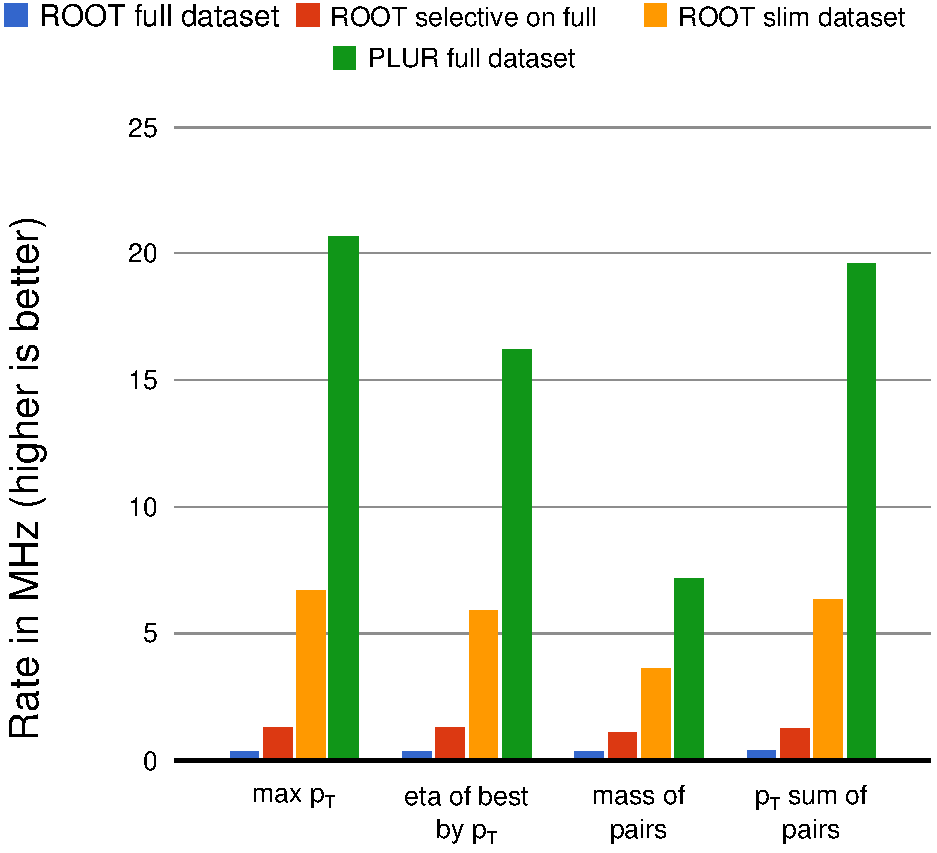
\includegraphics[width=\linewidth]{root-and-plur.pdf}}
%% \only<3->{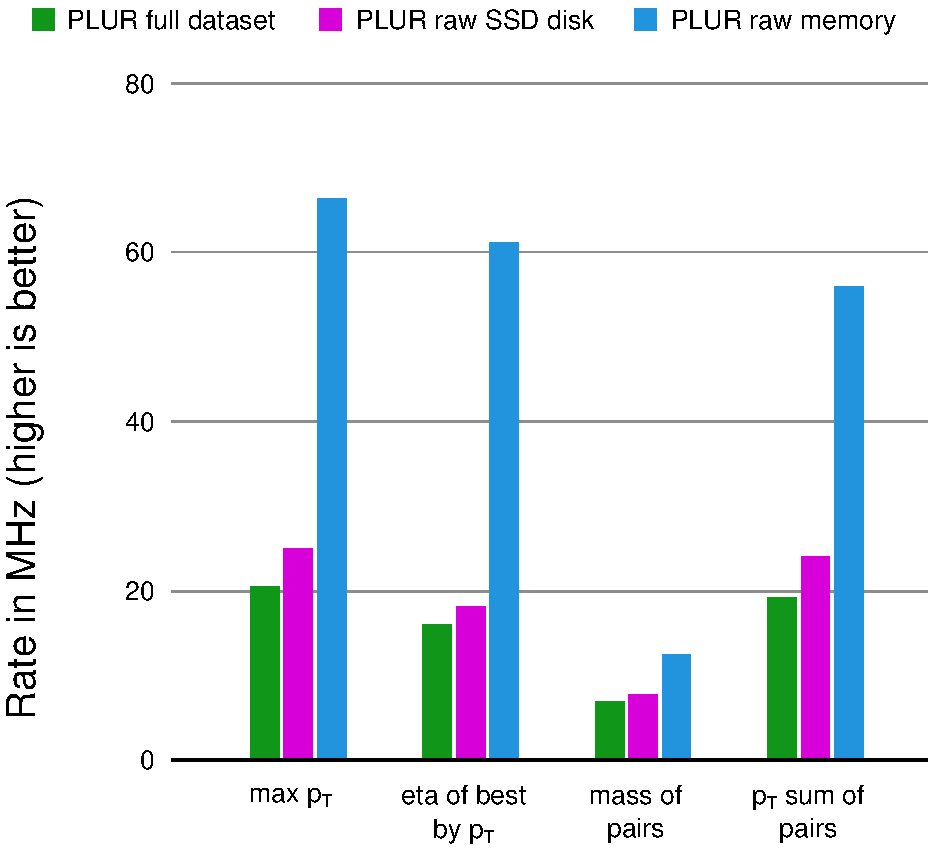
\includegraphics[width=\linewidth]{physical-media.pdf}}
\end{columns}
\end{uncoverenv}

\vspace{0.35 cm}
\begin{uncoverenv}<3->
Submitted to \href{http://cci.drexel.edu/bigdata/bigdata2017/index.html}{\textcolor{blue}{IEEE Big Data}}; subject of my \href{https://thestrangeloop.com/2017/particle-physics-10-000-times-faster.html}{\textcolor{blue}{StrangeLoop talk}}.
\end{uncoverenv}
\end{frame}

\begin{frame}[fragile]{Sharing data among versions}
\vspace{0.5 cm}
With an open API for {\it managing} data with columnar granularity (\href{https://github.com/diana-hep/plur}{\textcolor{blue}{see PLUR project}}), new versions of data structures can be produced without modifying or copying the original data.

\vspace{0.5 cm}
\begin{uncoverenv}<2->
For instance, a flat list of events

{\scriptsize\begin{verbatim}
      [Event, Event, Event,         Event, Event, Event, Event]
\end{verbatim}}

can be turned into a nested list of lumi blocks that partition events

{\scriptsize\begin{verbatim}
[Lumi([Event, Event, Event]), Lumi([Event, Event, Event, Event])]
\end{verbatim}}

{\it without touching the Event columns!} \textcolor{gray}{(Only adding Lumi columns, including an offset array to {\it conceptually} restructure the events.)}
\end{uncoverenv}

\vspace{0.5 cm}
\begin{uncoverenv}<3->
\fbox{\begin{minipage}{\linewidth}Users can correct jet energies, add reconstructed candidates, link gen and reco, skim particles, events, etc., all without modifying or copying--- so that dataset versions can share content like git. \end{minipage}}
\end{uncoverenv}
\end{frame}

\begin{frame}{Database indexing}
\vspace{0.5 cm}
\begin{columns}[c]
\column{0.6\linewidth}
Collaboration with \href{http://www.cdm.depaul.edu/about/Pages/People/facultyinfo.aspx?fid=1328}{\textcolor{blue}{Tanu Malik}}, database expert in the CS department at DePaul.

\vspace{0.2 cm}
In particular, she's interested in the idea of applying database-style indexes to {\it hierarchical} (non-tabular) data.

\column{0.3\linewidth}
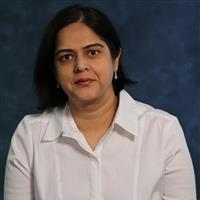
\includegraphics[width=\linewidth]{tanu.jpg}
\end{columns}

\vspace{0.5 cm}
\begin{uncoverenv}<2->
{\bf Some ideas:}
Approximate indexing with zonemaps and bitmaps, sorting events to concentrate high-$p_T$ in fewer disk pages\ldots
\end{uncoverenv}

\vspace{0.5 cm}
\begin{uncoverenv}<3->
\begin{minipage}{\linewidth}
{\bf Tanu found prior art in the literature:}

\scriptsize
Toni Mattis, Johannes Henning, Patrick Rein, Robert Hirschfeld, and Malte Appeltauer. 2015. {\it Columnar objects: improving the performance of analytical applications.} \\ DOI: \href{http://dx.doi.org/10.1145/2814228.2814230}{\textcolor{blue}{http://dx.doi.org/10.1145/2814228.2814230}}
\end{minipage}

\vspace{0.1 cm}
(But it doesn't do code transformation or database-style indexing.)
\end{uncoverenv}

\begin{uncoverenv}<4->
We're also writing a \href{https://docs.google.com/document/d/1-ZrnsS3IZdH91_pb99OLGd4gxaMm3m3Vr7XBigpx8DE/edit?usp=sharing}{\textcolor{blue}{community whitepaper}} on these topics.
\end{uncoverenv}
\end{frame}

\begin{frame}{Goals for columnar computing}
\vspace{0.2 cm}
\begin{block}{Short term ($\sim$few weeks)}
Finish the ``PLUR'' tools for physicists to run Python functions on their local, skimmed data faster than conventional C++ methods ({\tt\small SetBranchAddress/GetEntry}).
\begin{itemize}
\item Read ROOT with Brian's BulkIO through my \mbox{Numpy interface.\hspace{-1 cm}}
\item New columns, and someday database indexes, in SSD cache.
\item Transform Python code with PLUR, compile with Numba.
\item Use BulkIO/PLUR-friendly data tiers like CMS's NanoAOD.
\end{itemize}
\end{block}

\vspace{-0.2 cm}
\begin{uncoverenv}<2->
\begin{block}{Long term ($\sim$1 year)}
Demonstrator of a HEP query service: physicists submit Python code to a server, it runs on many nodes in parallel and returns small objects (histograms). Should be $\mathcal{O}({\mbox{1 second}})$ to be a reasonable competitor to local skims.
\begin{itemize}
\item working with Oli and Igor, incorporating ideas from Thanat's summer study, still hoping to work with off-the-shelf pieces\ldots
\end{itemize}
\end{block}
\end{uncoverenv}
\end{frame}

\begin{frame}{Contributions to ROOT and CMS}
\vspace{0.5 cm}
\textcolor{darkblue}{ROOT: Numpy interface on top of BulkIO}
\begin{itemize}
\item Gets data into Scientific Python libraries (Pandas, machine learning) more rapidly, not only PLUR.
\item Full integration with PyROOT (done).
\item High-level connectors to common Python libraries (planned).
\end{itemize}

\vspace{0.5 cm}
\begin{uncoverenv}<2->
\textcolor{darkblue}{CMS: Testing CMS NanoAOD}
\begin{itemize}
\item To ensure it's BulkIO-capable and PLUR-capable.
\item Performance-testing NanoAOD with BulkIO, \mbox{compression (LZ4),\hspace{-1 cm}} \\ and other experimental features like Brian's offset removal. Useful feedback to both NanoAOD group and ROOT I/O.
\item It would be great if there was a similar movement in ATLAS; the DxAODs are all {\tt\small std::vectors} (destructively serialized, yet with the same semantic information as a {\tt\small TLeaf[N]}).
\end{itemize}
\end{uncoverenv}
\end{frame}

\begin{frame}{Alternative ROOT reader}
\vspace{0.5 cm}
The BulkIO-Numpy API is simple enough (no streamers or classes) that it can be implemented in pure Python, without ROOT as a dependency.

\begin{center}
\href{https://github.com/scikit-hep/uproot}{\textcolor{blue}{https://github.com/scikit-hep/uproot}}

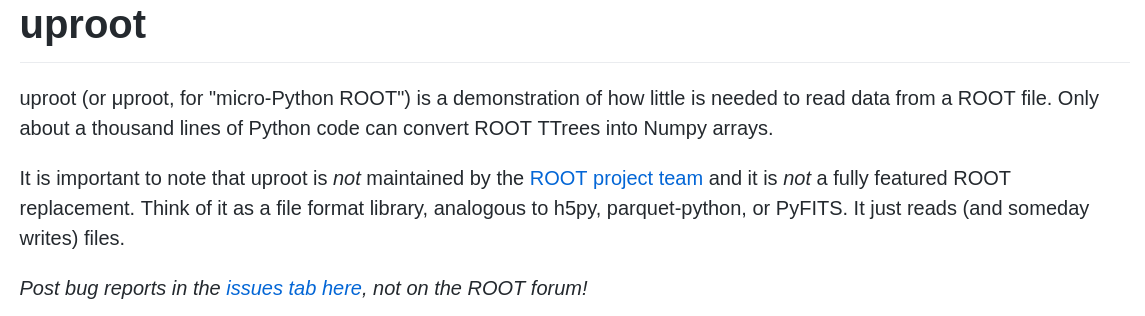
\includegraphics[width=0.9\linewidth]{uproot.png}
\end{center}

\begin{minipage}{\linewidth}
\small
\begin{enumerate}
\item View whole ROOT file as a memory-mapped array for rapid seeking.
\item Find bytes corresponding to basket data and cast as Numpy arrays.
\item Similar performance as BulkIO (same technique), but \mbox{easier to install.\hspace{-1 cm}}
\item Small scope: just reading simple leaves, mirroring \mbox{ROOT-Numpy API.\hspace{-1 cm}}
\end{enumerate}
\end{minipage}
\end{frame}

\begin{frame}{Conclusions}
\vspace{0.5 cm}
I'm working on many different projects, with many different people, but these projects are all connected: we're developing a high-level analysis environment with a performance {\it gain}, not a cost.

\vspace{0.5 cm}
\uncover<2->{Staged approach: first developing tools for analysts to use on their existing skims, then providing the same interface in a distributed service, then vectorization/type-checking gains from Femtocode.}

\vspace{0.5 cm}
\uncover<3->{Combination of uproot (for BulkIO-Numpy style interface), PLUR, and Histogrammar should be physicist-ready in weeks, maybe a month. Then I'll respond to feedback and iterate.}
\end{frame}

\end{document}
